\documentclass[12pt]{article}
\usepackage[margin=1in]{geometry}
\usepackage{times}
\usepackage[T1]{fontenc}
\usepackage[utf8]{inputenc}
\usepackage{amsmath,amssymb}
\usepackage{booktabs}
\usepackage{graphicx}
\usepackage{subcaption}
\usepackage{parskip}
\usepackage[numbers,sort&compress]{natbib}
\usepackage{hyperref}
\usepackage{stmaryrd}
\usepackage[font=small]{caption}

\pagestyle{empty}
\setlength{\abovedisplayskip}{6pt}
\setlength{\belowdisplayskip}{6pt}

\begin{document}

\noindent\textbf{\large From Controversy to Consensus: Modelling Community-Sensitive Common Ground Management in German Discourse Markers}

%\smallskip
%\noindent Hening Wang, Yuhan Guo \hfill \textit{Sinn und Bedeutung 30}
%\medskip

This study investigates three German discourse markers, which we label \emph{consensus markers} --- \textit{soviel ich wei\ss} (`as far as I know'), \textit{ja} (`roughly as you know'), and \textit{bekanntlich} (`as is well known') that differ in the strength of consensus marking: ranging from weak epistemic constraint (\textit{soviel ich weiß}) to strong public accessibility (\textit{bekanntlich}). 
These markers are functionally similar: they mark a proposition $p$ as uncontroversial \citep{zimmermann2011discourse}, settled in the common ground \citep{repp2013common}, and can be used manipulatively to support downstream communicative goals such as convincing an interlocutor \citep{doring2016modal}, often in contexts involving causal relationships \citep{seemann2025}. 
However, previous work (cf.\ \citep{grosz2021discourse}) has mostly focused on \textit{ja} and adopts a categorical framing that leaves open how notions like controversy vary \emph{gradiently} across markers and interact with other contextual factors. 
Building on these insights, we propose a novel utility-based, noisy-threshold model within probabilistic pragmatics \citep{goodman2016pragmatic, franke2016probabilistic, degen2023rational} and validate it with three preregistered experiments in social communication settings where causal information is relevant for convincing others to adopt a recommendation.\footnote{\href{https://osf.io/8snhk/overview?view\_only=c11af15b84814625832957bd31f561bb}{Link to the pre-registration}}.
Our theoretical contributions are threefold: (i) marker choice reflects a trade-off between perceived controversy and speaker goal strength, formalized as a utility function; (ii) perceived controversy further decomposes into propositional and pragmatic components, capturing the intuition that some controversial statements are less controversial within a specific community; (iii) the resulting utility space is partitioned by noisy thresholds rather than categorical boundaries, allowing overlapping regions where the decision is not clear-cut (see Fig.\ \ref{fig:threshold}). 
Empirically, we show that both perceived controversy and speaker goal strength have main effect on the production and comprehension of consensus markers (Fig.\ \ref{fig:production}--\ref{fig:comprehension}). Moreover, in production, the effect of goal strength is attenuated under high controversy. In comprehension, the strong marker \textit{bekanntlich} may trigger pragmatic reactance \citep{Brehm1966-BREATO-2}: listeners recognize the increased argumentative pressure and resist it, leading to lower adoption compared to the weaker \textit{ja}. Overall, \textit{ja} and \textit{bekanntlich} function similarly --- both are modulated primarily by perceived controversy, supporting a gradient view of boundaries between them. Our noisy-threshold model, trained on production data and applied to comprehension, captures these patterns within a single framework.

\textbf{Model.}
Perceived controversy combines propositional and pragmatic components: $pc = pc_{\text{prop}} \cdot pc_{\text{prag}}$. Marker choice is governed by $U(pc, g) = -w_{pc} \cdot pc + w_g \cdot g - w_{int} \cdot pc \cdot g$, where $g$ is goal strength and the interaction term captures the cost of invoking consensus under high controversy. Each marker $u_i$ occupies a noisy interval $[\theta_i, \theta_{i+1})$ on the utility scale, with $P(u_i \mid pc, g) \propto \sigma(\lambda(U - \theta_i)) \cdot \sigma(-\lambda(U - \theta_{i+1}))$. A pragmatic listener inverts this model via Bayes' rule to infer $pc$ and $g$, and downstream adoption depends on the inferred values.

\textbf{Experiments and results.}
Three preregistered experiments validate the model (Fig.\ \ref{fig:overview}).
In production (Fig.\ \ref{fig:production}), $g$ increases marker strength ($0.28$, $P(>0) = 1$), $pc_{\text{prag}}$ decreases it ($-0.17$, $P(<0) = 0.98$), and their interaction is negative ($-0.22$, $P(<0) = 0.97$), as $w_{int}$ predicts.
In comprehension (Fig.\ \ref{fig:comprehension}), both \textit{ja} ($0.49$, $P(>0) = 1$) and \textit{bekanntlich} ($0.46$, $P(>0) = 1$) increase inferred $g$, but only \textit{ja} boosts adoption credibly ($0.42$, $P(>0) = 0.99$; \textit{bekanntlich}: $0.17$, $P(>0) = 0.90$). The marker-by-controversy interactions point in opposite directions for both inferences: for $g$, the \textit{ja} effect trends larger under high controversy ($0.28$, $P(>0) = 0.95$); for adoption, smaller ($-0.31$, $P(<0) = 0.93$) --- consistent with pragmatic reactance.

% ============================================================
% PAGE 2: FIGURES
% ============================================================
\clearpage

\begin{figure}[h!]
  \centering
  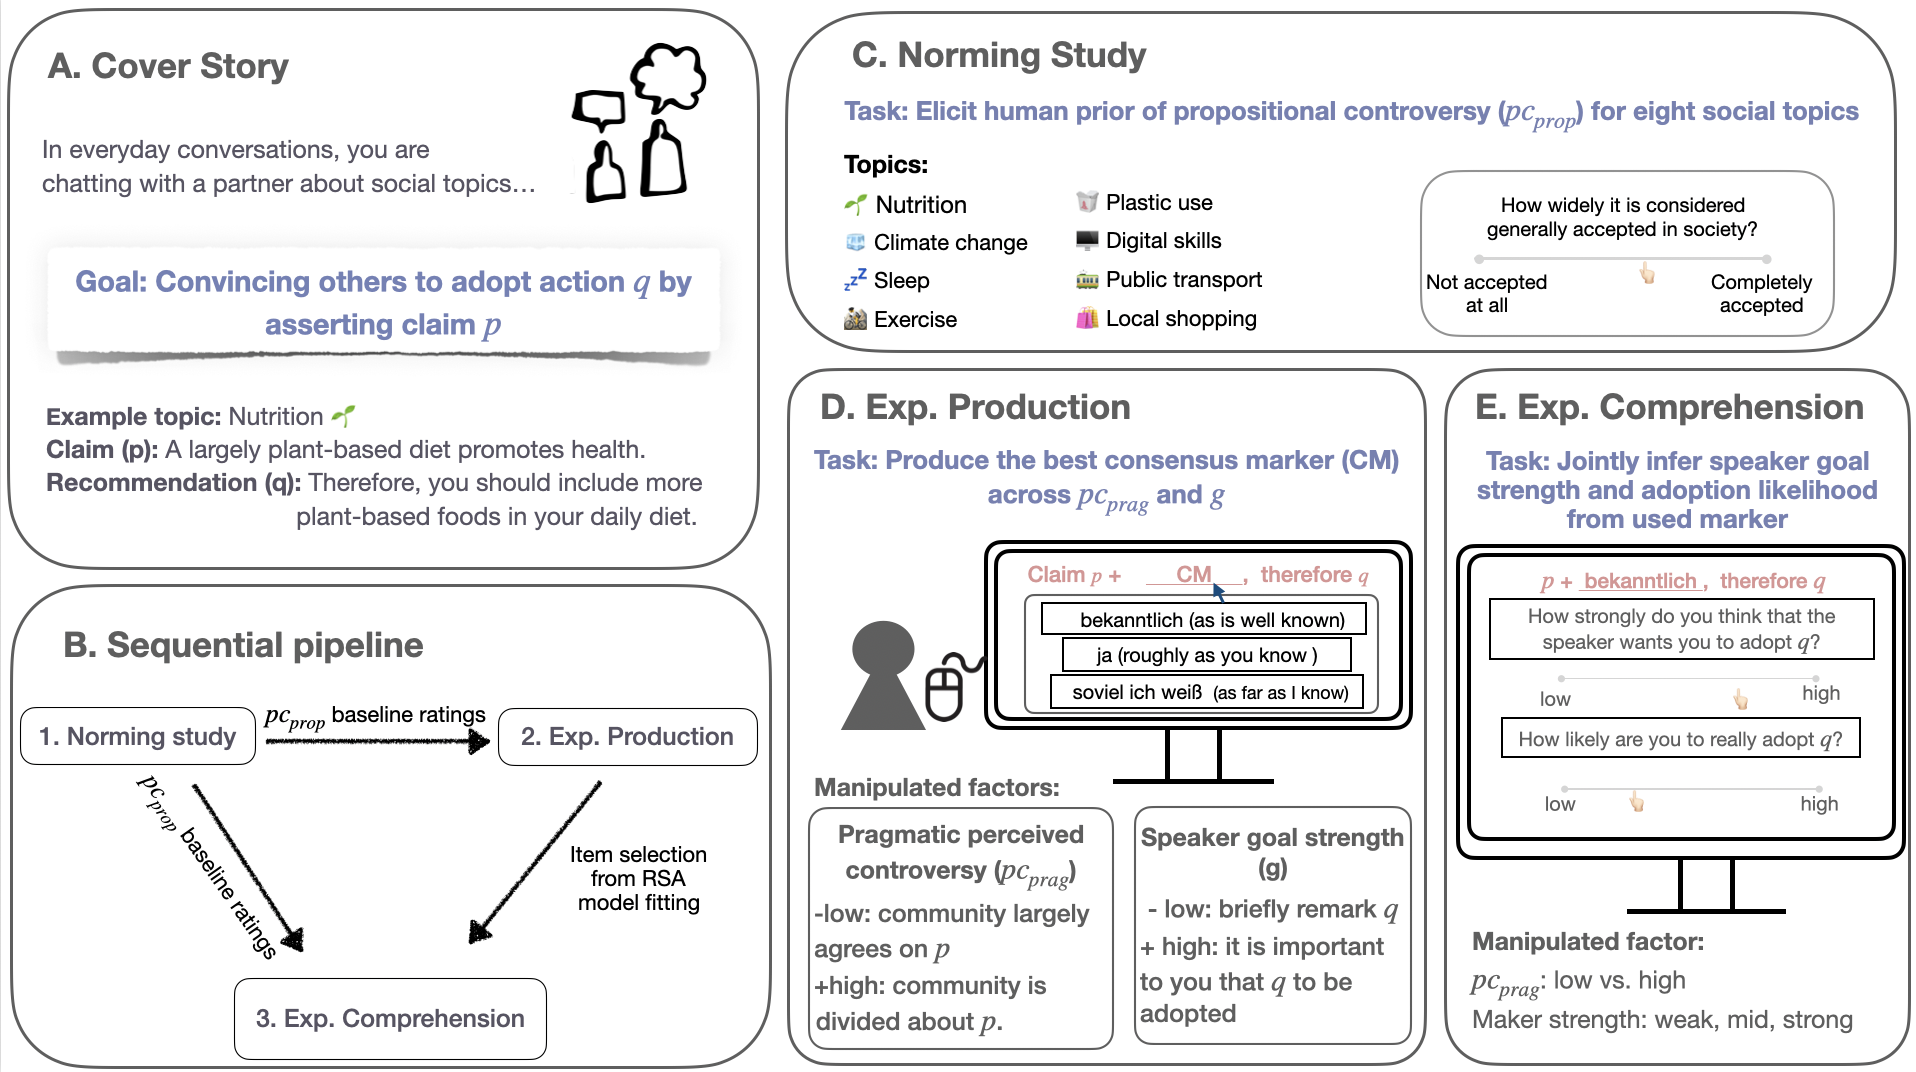
\includegraphics[width=0.6\textwidth]{overview.png}
  \caption{Experimental pipeline. (A)~Cover story: participants discuss social topics with a partner, aiming to convince them to adopt a recommendation. (B)~Sequential design: a norming study establishes baseline propositional controversy, followed by production and comprehension experiments. (C)~Norming: eight topics rated for propositional controversy. (D)~Production: participants select the best consensus marker given manipulated pragmatic controversy and goal strength. (E)~Comprehension: participants infer speaker goal strength and adoption likelihood from marker-containing utterances.}
  \label{fig:overview}
\end{figure}

\begin{figure}[h!]
  \centering
  \begin{subfigure}[b]{0.45\textwidth}
    \centering
    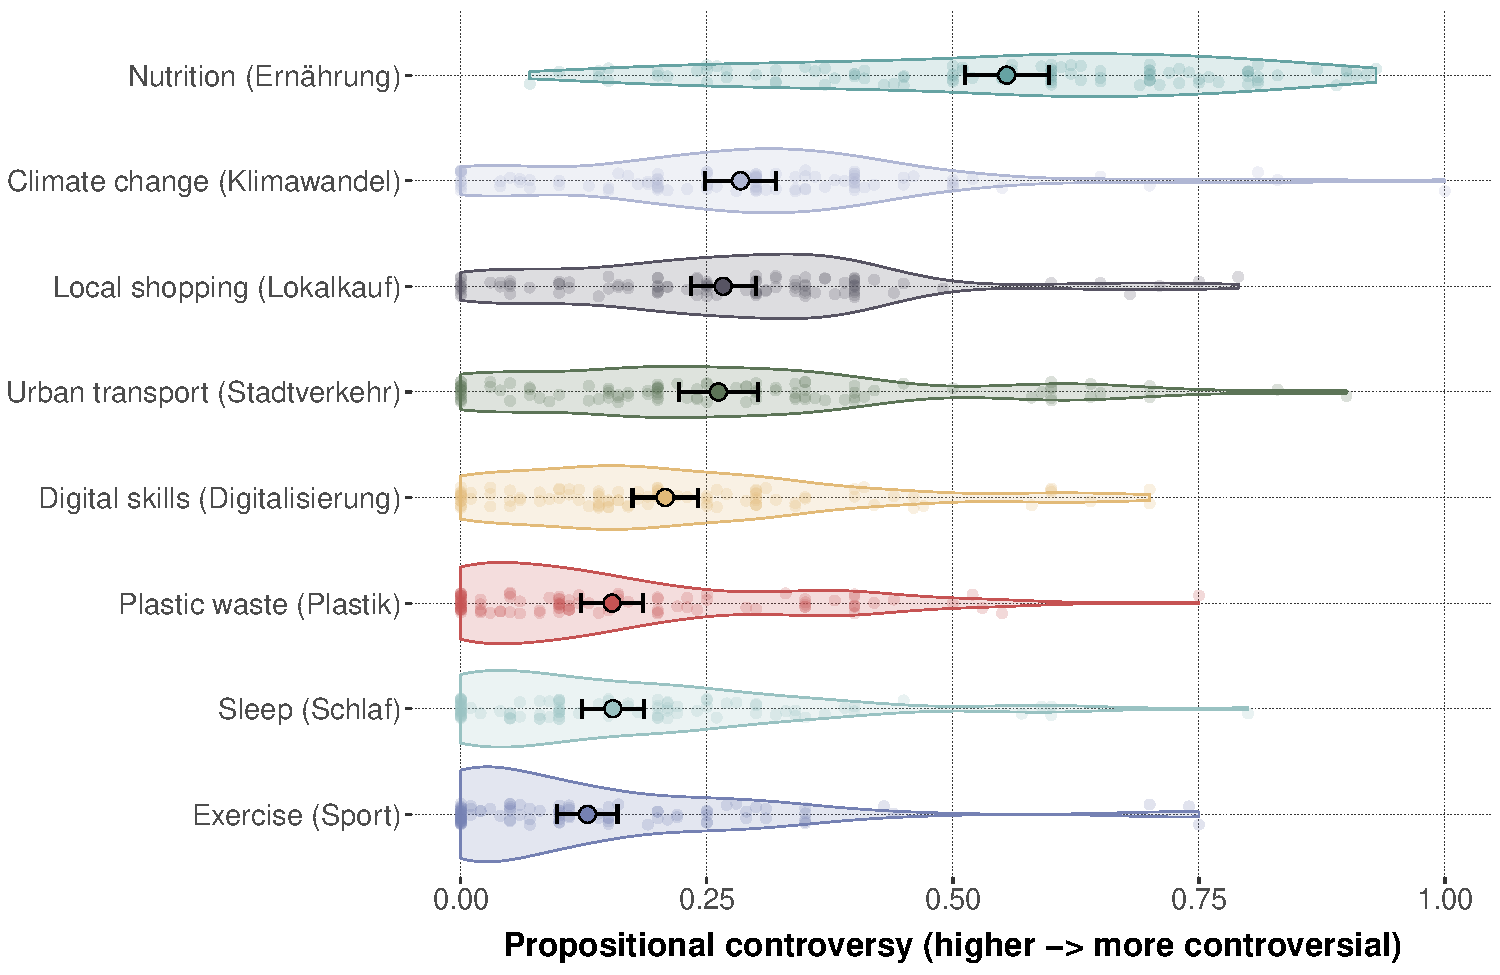
\includegraphics[width=\textwidth]{fig_norming.pdf}
    \caption{Results of the norming experiment ($N\!=\!102$).}\label{fig:norming}
  \end{subfigure}\hfill
  \begin{subfigure}[b]{0.45\textwidth}
    \centering
    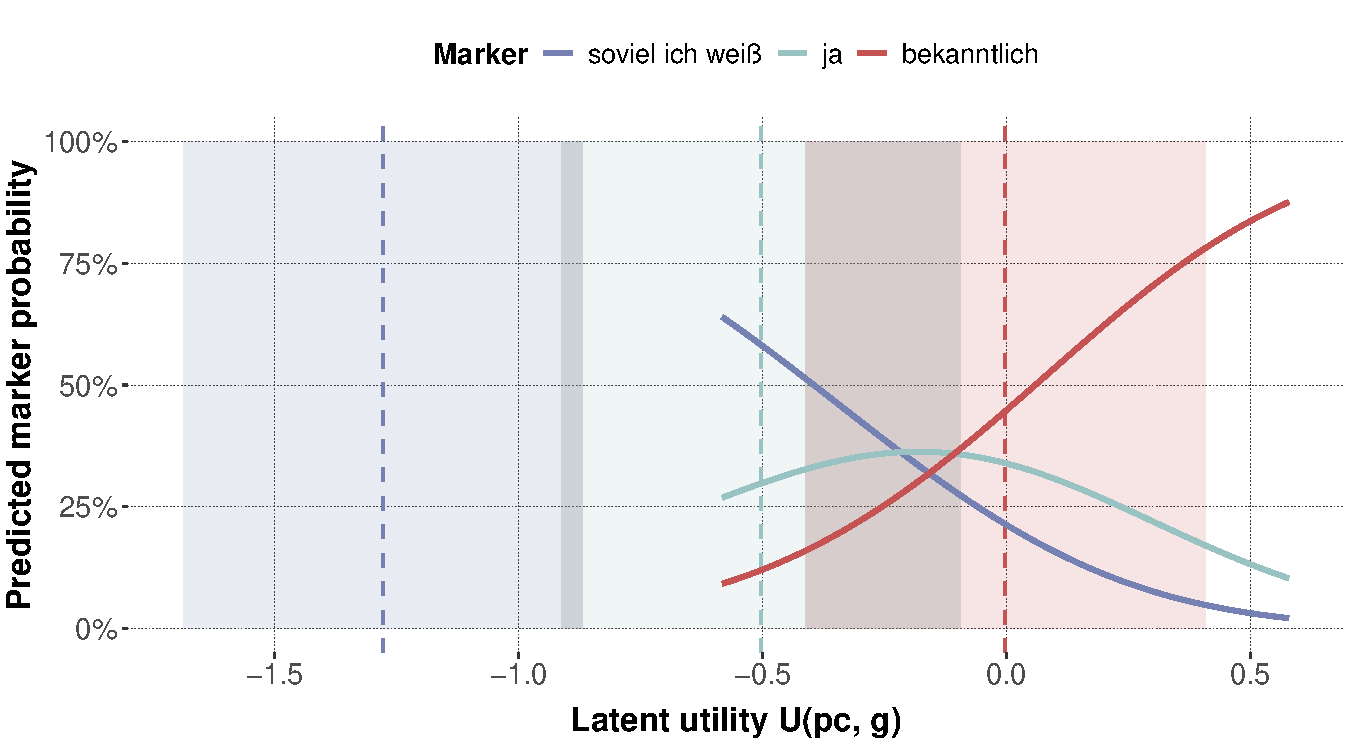
\includegraphics[width=\textwidth]{fig_rsa_thresholds.pdf}
    \caption{RSA noisy thresholds along the latent utility axis. Dashed lines: mean thresholds; shaded bands: overlapping regions.}\label{fig:threshold}
  \end{subfigure}

  \smallskip

  \begin{subfigure}[b]{0.45\textwidth}
    \centering
    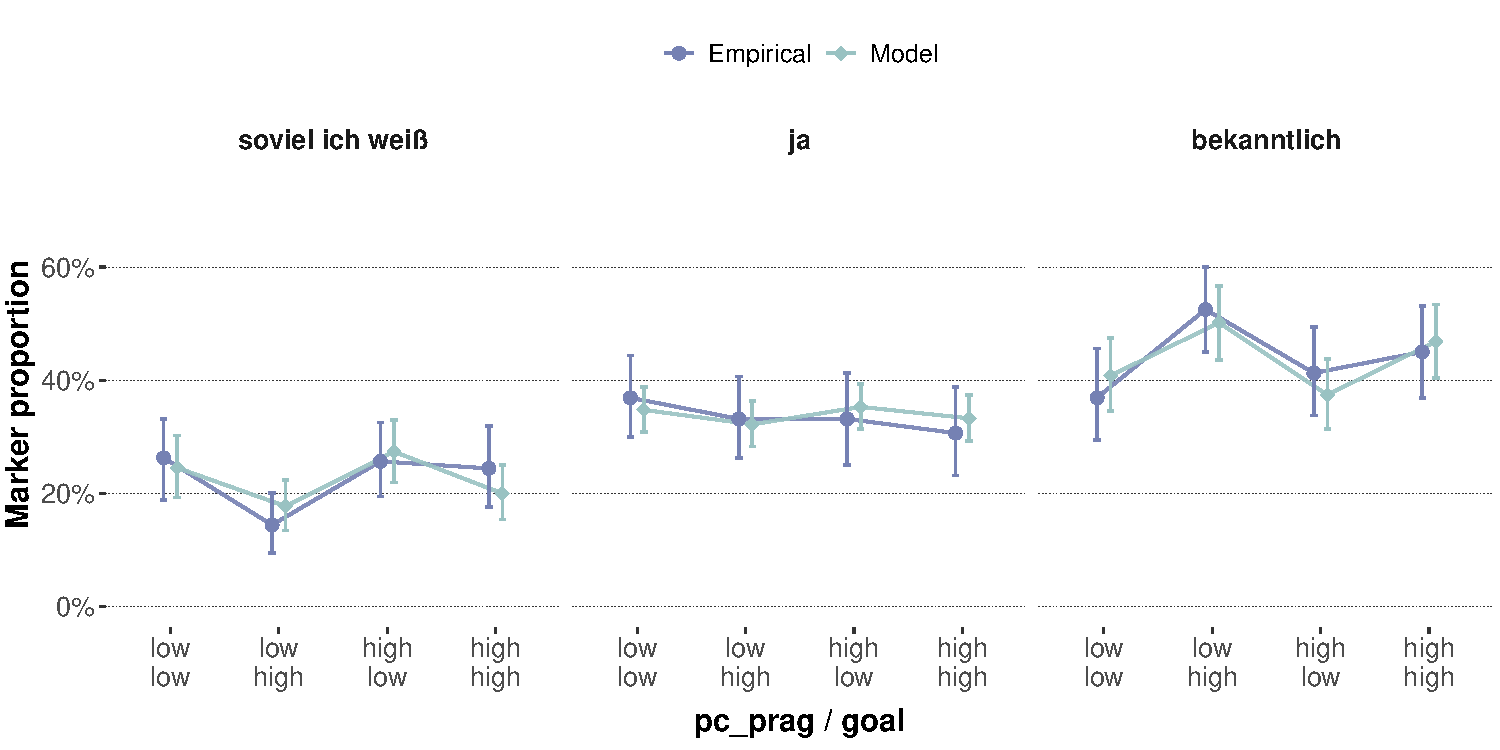
\includegraphics[width=\textwidth]{../../analysis/production_exp/plots/fig17c_facet_by_marker.pdf}
    \caption{Results of the production experiment ($N\!=\!80$).}\label{fig:production}
  \end{subfigure}\hfill
  \begin{subfigure}[b]{0.45\textwidth}
    \centering
    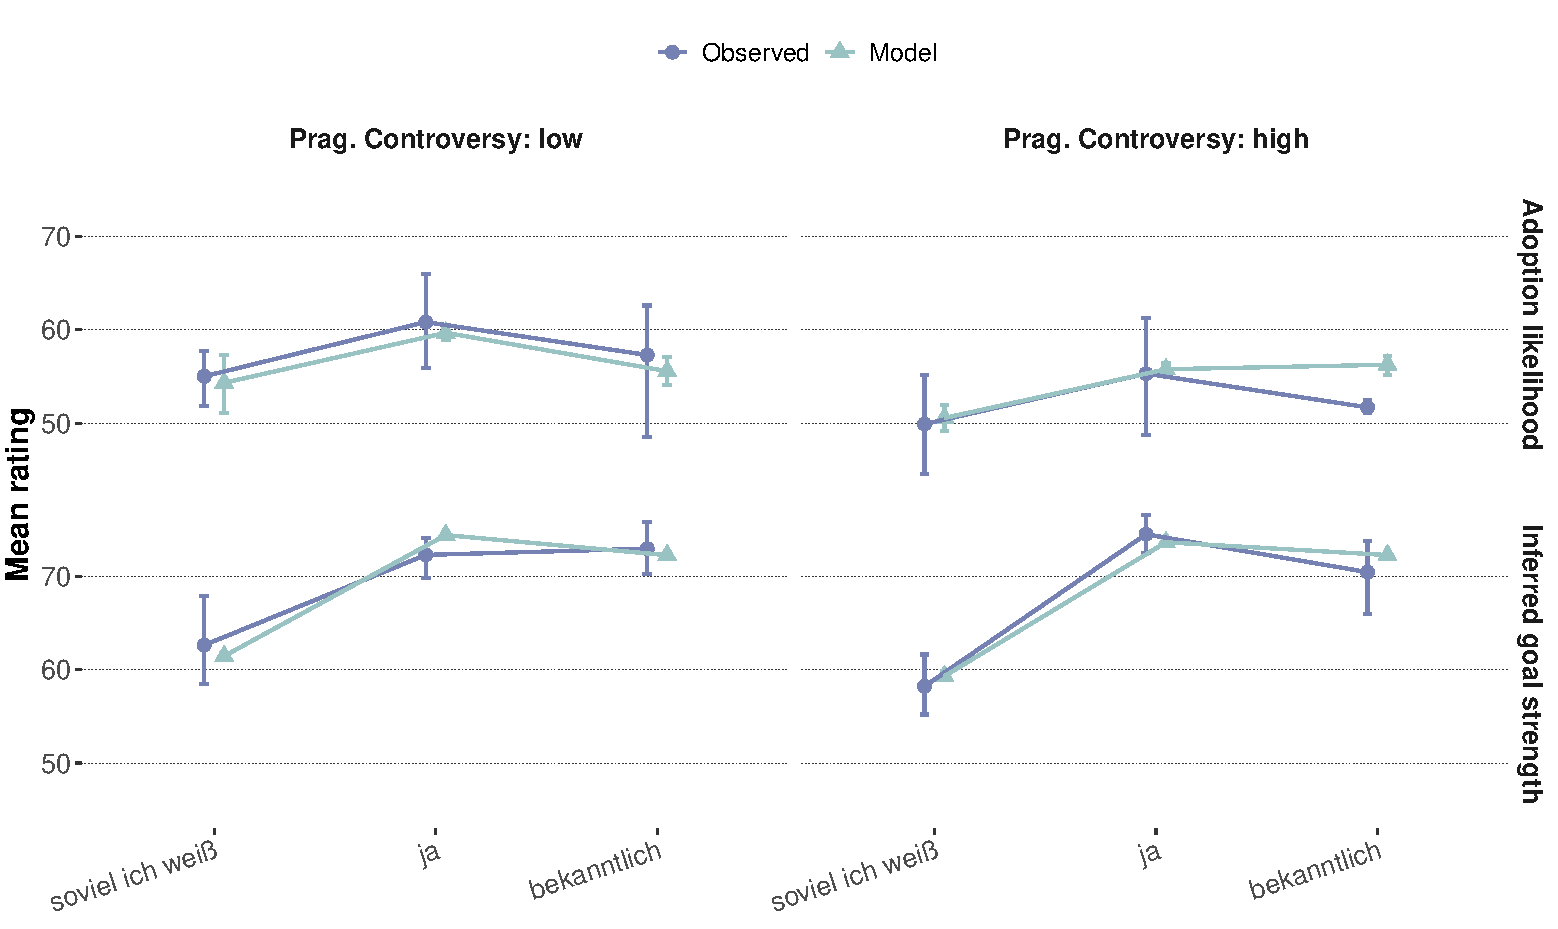
\includegraphics[width=\textwidth]{../../analysis/comprehension_exp/plots/fig7_rsa_base_vs_enhanced.pdf}
    \caption{Results of the comprehension experiment ($N\!=\!80$).}\label{fig:comprehension}
  \end{subfigure}

  \caption{Model and experimental results. Points show means; error bars show bootstrap 95\% confidence intervals.}
  \label{fig:all-results}
\end{figure}
\clearpage
\newpage
\textbf{References:}
\renewcommand{\bibsection}{}
{\footnotesize
\bibliographystyle{unsrtnat}
\bibliography{references}
}
\end{document}
